\documentclass[12pt]{constitution}

\usepackage{mathpazo}
\usepackage[frenchb]{babel}
\usepackage[T1]{fontenc}
\usepackage[utf8]{inputenc}
\usepackage{array, multirow, tabularx}
\usepackage{graphicx}
\usepackage{multicol}

\begin{document}

\title{Convention entre l'Association de Gestion de la Résidence et le Rézoléo}
\author{Association Rézoléo - Association de Gestion de la Résidence}
\date{01/09/2017}
\maketitle

\section{Objet de la convention}

    La présente convention a pour objet de définir les relations concernant la gestion et l'accessibilité du réseau local de la Résidence Léonard de Vinci (désignée ci-dessous par "la Résidence") et le partage effectif des responsabilités entre l'Association de Gestion de la Résidence (désignée ci-dessous par "AGR") et le Rézoléo, association type Loi 1901, déclarée en préfecture du Nord.


\section{Modalités d'application de la convention}

    La convention est convenue et signée pour 3 ans. Elle est modifiable par avenant à la demande d'une des deux parties. L'AGR s'engage à respecter le terme des 3 ans sauf violation d'une des dispositions de la présente convention par une des deux parties.


\section{Engagements du Rézoléo}

    Le Rézoléo est une association gérée par les résidents de la Résidence Léonard de Vinci, qui assure bénévolement la maintenance et l'accès aux services permis par le réseau informatique de la Résidence. À ce titre, le Rézoléo raccorde ses adhérents connectés au réseau local de la Résidence. Ce service est assuré de manière bénévole par des élèves qui s'y engagent librement, et peuvent à tout moment et sans risque de sanctions renoncer à cette responsabilité.\\


    Le Rézoléo s'engage à pourvoir aux obligations prévues par la loi dans le cadre de la seule exploitation technique du réseau informatique. À ce titre, le Rézoléo s'engage à garder trace des noms des usagers, des heures de connexion, des adresses IP et des caractéristiques de leurs appareils pour une durée de 1 an. Conformément à la loi relative à l'informatique, aux fichiers et aux libertés, le Rézoléo ne conserve aucune trace portant sur le contenu des correspondances ou sur les informations consultées. Le Rézoléo est responsable de la confidentialité de ces données conservées et du bon respect des prérogatives de la CNIL.\\


    Le Rézoléo s'occupe également de résoudre les problèmes que peut rencontrer le réseau, qu'il s'agisse de défaillances physiques ou bien d'attaques informatiques.\\

    En cas de risque majeur pour l'intégrité du réseau de la Résidence, le Président du Rézoléo s'engage à en avertir dans les plus brefs délais un représentant de l'AGR. Il proposera si possible un diagnostic du problème rencontré et des moyens nécessaires pour le corriger.\\


    Le Rézoléo notifie une semaine à l'avance toute intervention sur l'électricité ou les fluides dans les locaux.\\


    Le Rézoléo raccorde gratuitement l'ensemble du matériel de l'AGR au réseau local.\\


    En dehors d'un cas avéré de négligence ou de malveillance, l'AGR ne peut pas tenir le Rézoléo responsable des conséquences de tout mauvais diagnostic concernant un problème qui aurait été effectué par un membre du Rézoléo.


\section{Engagements de l'AGR}

     L'AGR facilitera les activités du Rézoléo dans la mesure de ses moyens. L'AGR fournira au Rézoléo les accès nécessaires aux différents locaux selon les modalités spécifiées en annexe.\\


    L'AGR s'engage à prévenir, 48 heures à l'avance dans la mesure du possible, le Rézoléo de toute opération sur le réseau électrique pouvant impacter les services proposés à ses adhérents.\\


    L'AGR s'engage à fournir une réponse sous 2 semaines à toute demande d'intervention de la part du Rézoléo.\\


    L'AGR avise le Rézoléo de tout mouvement dans l'attribution des chambres au sein de la Résidence, pour permettre une gestion rigoureuse des propriétaires de chaque connexion.\\

\section{Locaux}

    Dans le but d'assurer la pérennité de l'association Rézoléo, le local LCR D3 est un espace de formation de ses parties bénévoles, notamment à la gestion et à l'administration d'un réseau informatique.\\

    De plus l'AGR s'engage à fournir au Rézoléo un accès physique à tous les locaux où il peut être amené à intervenir.\\

    Le rézoléo fournit en début de chaque année scolaire la liste des locaux auxquel il souhaite avoir accès.\\
    
\section{Propriété du matériel}

    L'AGR est propriétaire des switchs des locaux techniques, des baies de brassage, de l'ensemble du câblage de la Résidence à l'exception de l'ensemble des équipements achetés par le Rézoléo depuis le début de son activité.\\

    Les serveurs, outillage de maintenance, le matériel informatique situés en dehors des locaux techniques sont la propriété du Rézoléo.


\section{Période d'essai}

    L'AGR s'engage à laisser une période d'essai de trois ans au Rézoléo après raccordement de la Résidence par le Fournisseur d'Accès à Internet Quantic Telecom. Cette période d'essai passée, l'AGR se réserve le droit, si le Rézoléo se soustrait à ses obligations de moyens, de récupérer la gestion exclusive du réseau de la Résidence avec un préavis de 3 mois.\\

    Le Rézoléo s'engage suite à sa période d'essai à racheter progressivement, dans la mesure du possible, l'ensemble des équipements informatiques mis à disposition par l'AGR, en prenant en compte l'amortissement de ceux-ci. Les locaux techniques pourront être loués par l'AGR au Rézoléo.\\


\section{Litiges et rupture de la convention}

    En cas de litige, les parties s'accordent pour tenter de résoudre ce dernier à l'amiable. Dans le cas où aucun accord ne pourrait être trouvé, les parties porteront l'affaire devant les juridictions territorialement compétentes.


    Le Rézoléo s'engage en tout état de cause, si l'association arrête l'exploitation des réseaux des Résidences de l'AGR, de prévenir au moins trois mois à l'avance la direction d'AGR de cette décision par courrier recommandé et lettre simple, afin de permettre à l'AGR d'assurer la continuité du service au bénéfice des résidents par son propre réseau.\\

Fait à Villeneuve D'Ascq le .............\\


\noindent Signatures \\
Président du Rézoléo \hfill Représentant de l'AGR

    \newpage

    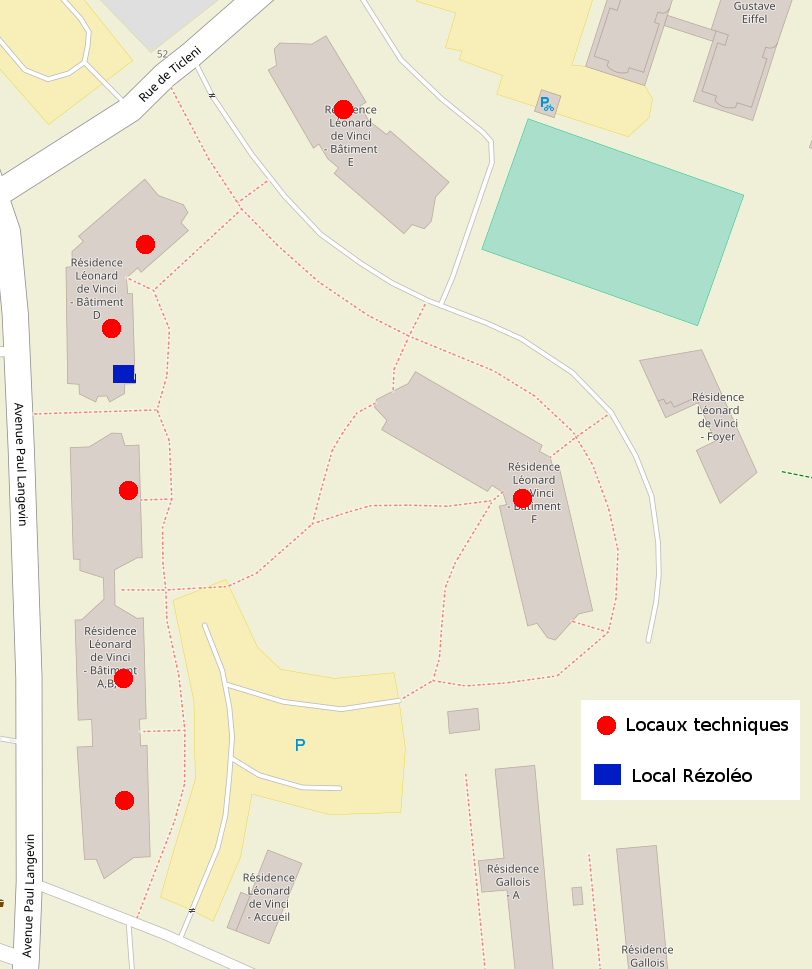
\includegraphics[scale=0.6]{carteLocaux.png}

\end{document}
